En esta secci\'on se presentan algunos ej\'emplos de programas con el resultado correspondiente.

\subsection{Programas v\'alidos}

El siguiente ejemplo, es un ejemplo que se llego a correr para la primer entrega de este trabajo, por lo que es un buen ejemplo para ver la evoluci\'on del c\'odigo. \\
Primero se va a mostrar el ejemplo del programa que se va a ejecutar, luego el resultado del c\'odigo de la primer entrega, y despu\'es el resultado correspondiente al c\'odigo presentado en esta entrega.\\
Para ver la diferencia de forma m\'as clara la im\'agen de fondo negro es la presentada anteriormente, y de fondo blanca es la actual.\\

\lstinputlisting[breaklines=true]{../Ejemplos/eg04.peg}


\centerline{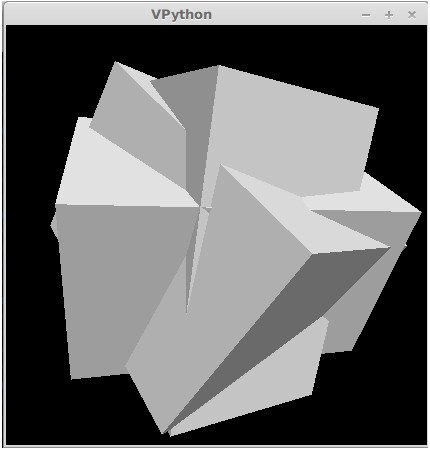
\includegraphics[scale=0.40]{../imagenes/eg04.jpg}}


\centerline{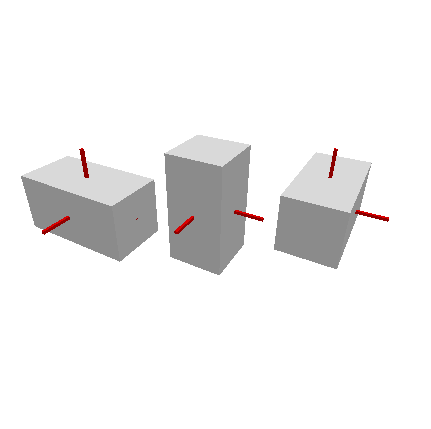
\includegraphics[scale=0.40]{../imagenes/eg04_nuevo.png}}


El ejemplo que se presenta a continuaci\'on, al igual que el anterior, se ejecut\'o con el c\'odigo de la entrega anterior y con el presentado en esta entrega. Por lo que tambi\'en se puede observar la diferencia entre ambos resultados.\\
Los mismos se presentan en el mismo orden correspondiente al ejemplo anterior.\\

\lstinputlisting[breaklines=true]{../Ejemplos/eg11.peg}


\centerline{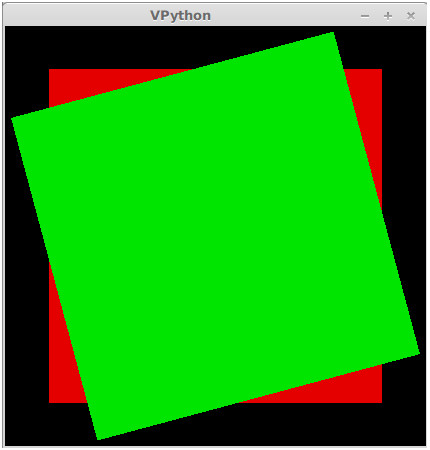
\includegraphics[scale=0.40]{../imagenes/eg11.jpg}}


\centerline{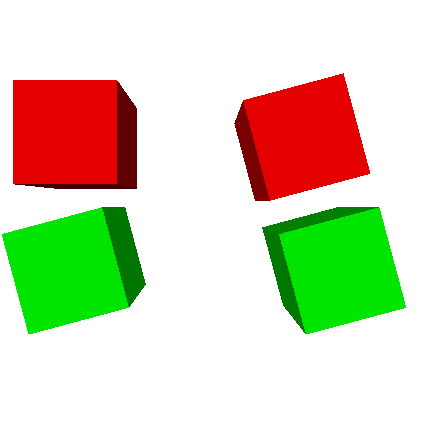
\includegraphics[scale=0.40]{../imagenes/eg11_nuevo.png}}

\newpage
Los siguientes ejemplos fueron ejecutados con el c\'odigo de esta entrega.\\
\lstinputlisting[breaklines=true]{../Ejemplos/eg22.peg}

\centerline{
\includegraphics[scale=0.40]{../imagenes/eg22.png}}


\lstinputlisting[breaklines=true]{../Ejemplos/eg23.peg}

\centerline{
\includegraphics[scale=0.40]{../imagenes/eg23.png}}



\lstinputlisting[breaklines=true]{../Ejemplos/eg24.peg}

\centerline{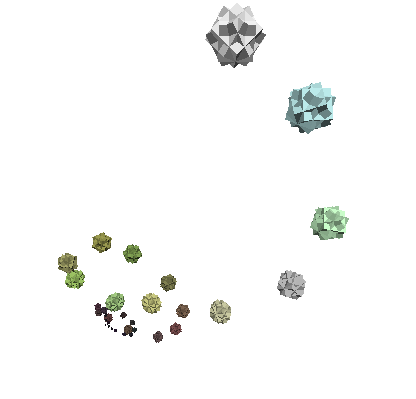
\includegraphics[scale=0.40]{../imagenes/eg24.png}}


\lstinputlisting[breaklines=true]{../Ejemplos/eg25.peg}

\centerline{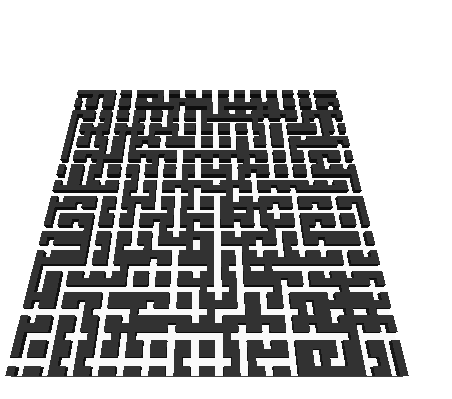
\includegraphics[scale=0.40]{../imagenes/eg25.png}}


\lstinputlisting[breaklines=true]{../Ejemplos/eg26.peg}

\centerline{
\includegraphics[scale=0.40]{../imagenes/eg26.png}}


\lstinputlisting[breaklines=true]{../Ejemplos/eg27.peg}

\centerline{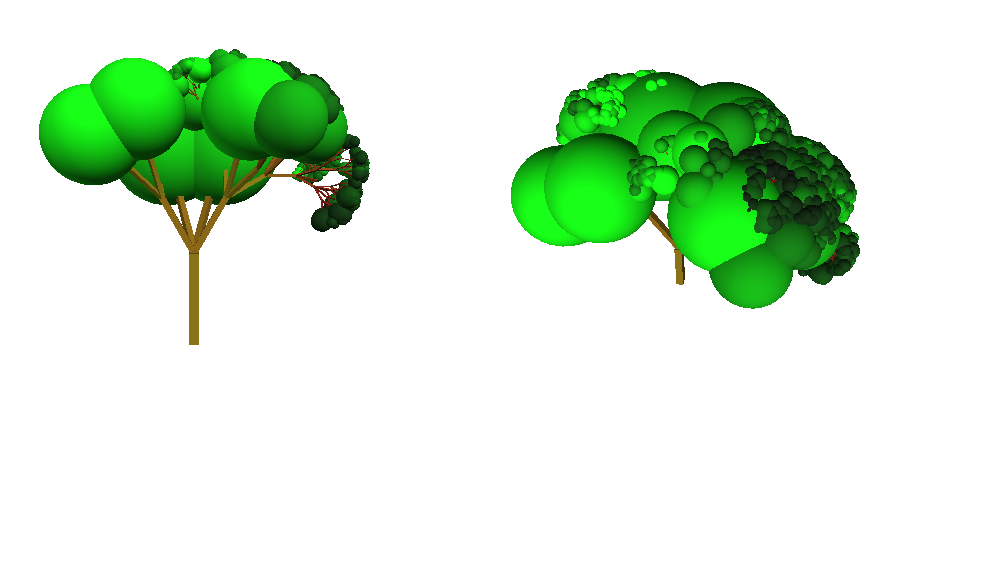
\includegraphics[scale=0.40]{../imagenes/eg27.png}}


\lstinputlisting[breaklines=true]{../Ejemplos/cara.peg}

\centerline{
\includegraphics[scale=0.40]{../imagenes/cara.png}}

\newpage

\subsection{Programas inv\'alidos}

\lstinputlisting[breaklines=true]{../Ejemplos/eg22invalid.peg}

\centerline{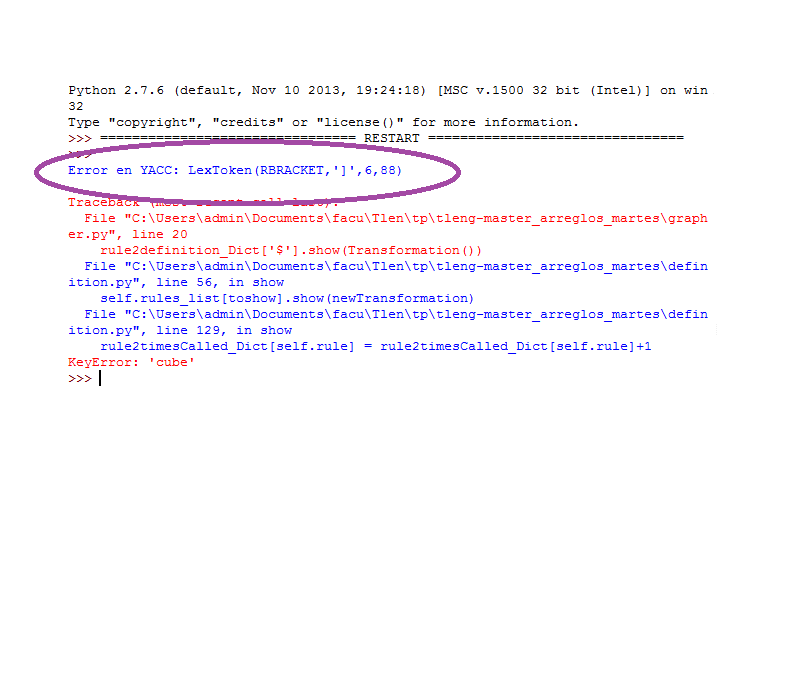
\includegraphics[scale=0.70]{../imagenes/eg22invalid.png}}

\lstinputlisting[breaklines=true]{../Ejemplos/eg22invalid2.peg}

\centerline{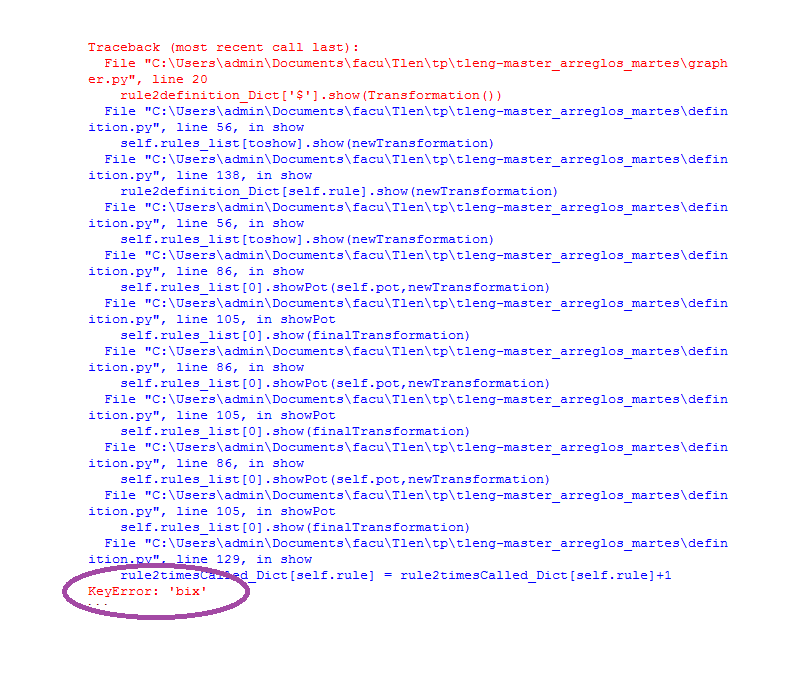
\includegraphics[scale=0.70]{../imagenes/eg22invalid2.png}}

\lstinputlisting[breaklines=true]{../Ejemplos/carainvalid.peg}

\centerline{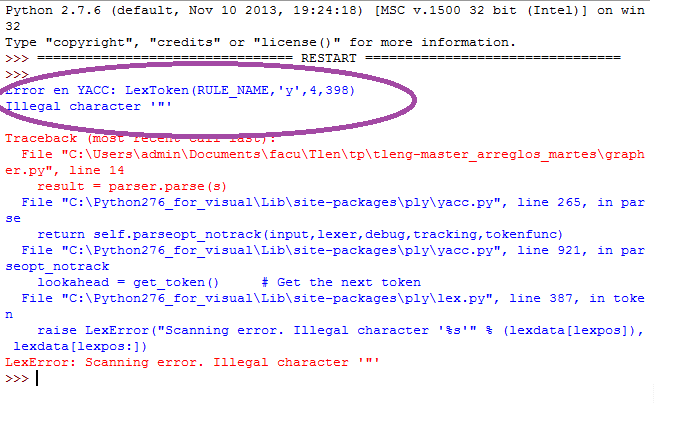
\includegraphics[scale=0.70]{../imagenes/carainvalid.png}}